% Chapter 2

\chapter{Literature Study} % Main chapter title

\label{Literature Study} % For referencing the chapter elsewhere, use \ref{Chapter1} 

%----------------------------------------------------------------------------------------

% Define some commands to keep the formatting separated from the content 

%----------------------------------------------------------------------------------------

\section{Knowledge Discovery Steps}

%----------------------------------------------------------------------------------------

\section{Data Mining Concepts}

\section{Preprocessing}

%----------------------------------------------------------------------------------------
\section{Classification}
\subsection{Basic Concept}

\paragraph{}Classification is a form of data analysis that extracts models describing important data classes. Such models,called classifiers, predict categorical (discrete, unordered) class labels. For example, we can build a
classification model to categorize bank loan applications as either safe or risky. Such analysis can help provide
us with a better understanding of the data at large. Many classification methods have been proposed by
researchers in machine learning, pattern recognition, and statistics. Most algorithms are memory resident,
typically assuming a small data size. Recent data mining research has built on such work, developing scalable
classification and prediction techniques capable of handling large amounts of disk-resident data. Classification
has numerous applications, including fraud detection, target marketing, performance prediction, manufacturing,
and medical diagnosis.

\paragraph{}
The data analysis task is classification, where a model or classifier is constructed to predict class (categorical) labels.This model is a predictor.Regression analysis is a statistical methodology that is most often used for numeric prediction; hence the two terms tend to be used synonymously, although other methods for numeric prediction exist. Classification and numeric prediction are the two major types of prediction problems.


\subsection{General Approach to Classification}
\paragraph{}
 Data classification is a two-step process, consisting of a learning step
(where a classification model is constructed) and a classification step (where the model is used to predict class
labels for given data).
\paragraph{}
In the first step, a classifier is built describing a predetermined set of data classes or concepts. This is the
learning step (or training phase), where a classification algorithm builds the classifier by analyzing or
"learning from" a training set made up of database tuples and their associated class labels. A tuple, $ X$, is
represented by an n-dimensional attribute vector, $ X= (x_{1},x_{2},....,x_{n})$ depicting n measurements made on the tuple from n database attributes, respectively,$A_{1},A_{2},....A_{n} $.\footnote{\label{first}Each attribute represents a "feature" of $X$. Hence, the pattern recognition literature uses the term feature vector rather than
attribute vector. } 
Each tuple, $X$, is assumed to belong to a predefined class as determined by another database attribute called the class label attribute. The class label
attribute is discrete-valued and unordered. It is categorical (or nominal) in that each value serves as a category
or class. The individual tuples making up the training set are referred to as training tuples and are randomly
sampled from the database under analysis. In the context of classification, data tuples can be referred to as
samples, examples, instances, data points, or objects.\footnote{\label{second}In the machine learning literature, training tuples are commonly referred to as training samples. Throughout this text, we prefer to use the term tuples instead of samples.}
\begin{figure}
   \centering
  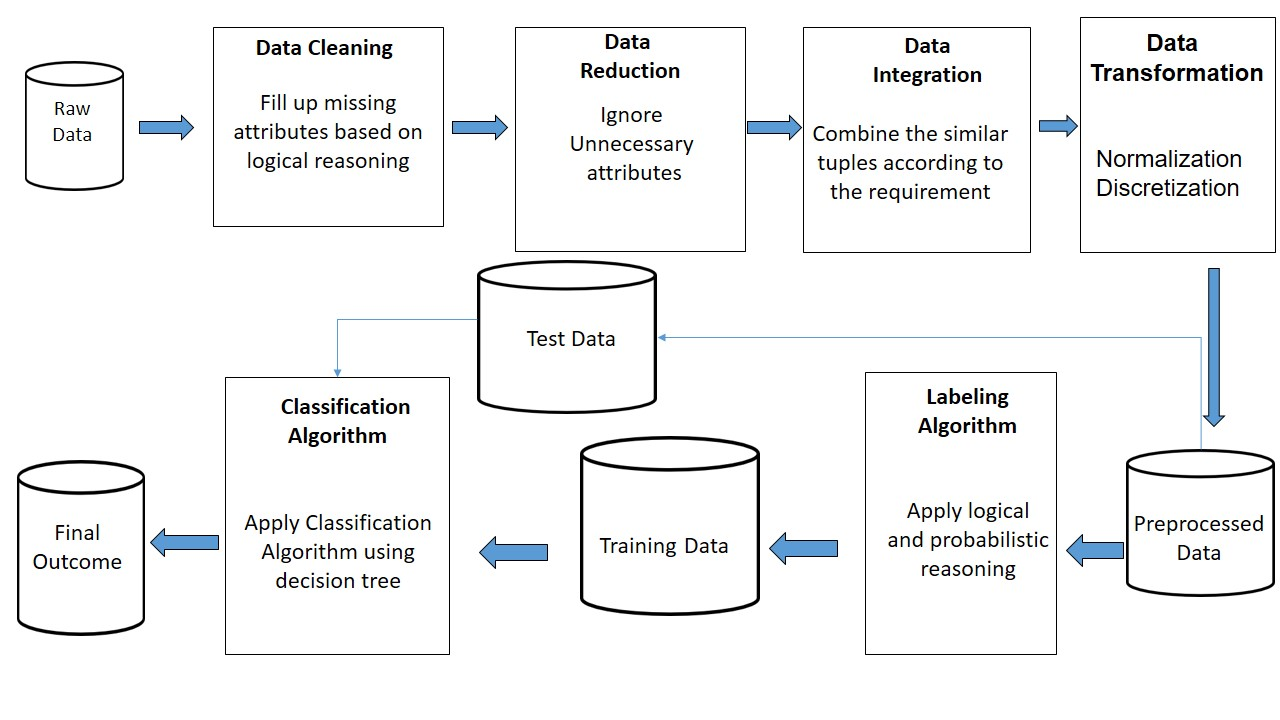
\includegraphics[width=\linewidth]{Figures/classification.jpg}
  \decoRule
  \caption[Classification]{General Process of Classification}
  \label{fig:classification}
\end{figure}

Figure ~\ref{fig:classification} shows the general procedure of classification.
\subsection{Decision Tree Induction}
\paragraph{}
Decision tree induction is the learning of decision trees from class-labeled training tuples. A decision tree is a
flowchart-like tree structure, where each internal node (nonleaf node) denotes a test on an attribute, each
branch represents an outcome of the test, and each leaf node (or terminal node) holds a class label. The
topmost node in a tree is the root node. 
The decision tree in Figure ~\ref{fig:decisiontree} is a tree for the concept buy\_computer that indicates whether a customer at a company is likely to buy a computer or not. Each internal node represents a test on an attribute. Each leaf node represents a class.
The benefits of having a decision tree are 
\begin{itemize}
\item It does not require any domain knowledge.
\item is easy to comprehend.
\item The learning and classification steps of a decision tree are simple and fast.
\end{itemize}
    

\begin{figure}
   \centering
  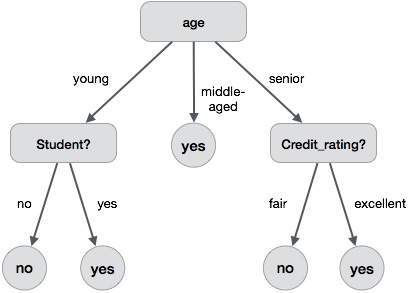
\includegraphics[width=\linewidth]{Figures/dm_decision_tree.jpg}
  \decoRule
  \caption[A Decision Tree]{A Decision Tree}
  \label{fig:decisiontree}
\end{figure}

\subsection{Decision Tree Induction Algorithm}
A machine researcher named J. Ross Quinlan in 1980 developed a decision tree algorithm known as ID3 (Iterative Dichotomiser). Later, he presented C4.5, which was the successor of ID3. ID3 and C4.5 adopt a greedy approach. In this algorithm, there is no backtracking; the trees are constructed in a top-down recursive divide-and-conquer manner.

\begin{algorithm}[H]

\label{generatedecisiontree}
\SetKwInOut{Input}{Input}
\SetKwInOut{Output}{Output}

\Input{ \begin{itemize}
\item Data partition, D, which is a set of training tuples and their associated class labels;
\item $attribute\_list$, the set of candidate attributes\;
\item $Attribute\_selection\_method $.
\end{itemize}}
\Output{A decision tree.}

\begin{algorithmic}[1]
\caption{Generate\_decision\_tree}
\Procedure{}{}
    \State create a node $N$\;
    \If{tuples in $D$ are all of the same class, $C$,}{
    	return $N$ as leaf node labeled with the class $C$ \;
    }
    
    \If{$attribute\_list$ is empty}{
    	return $N$ as leaf node labeled with the majority class in $D$ \;
    }
   \State apply $Attribute\_selecction\_method(D,attribute\_list)$ to find best splitting\-criterion \;  
        
   \State label node $N$ with $splitting_criterion$ \;
    \If{$splitting\_criterion$ is discrete valued and multiway splits allowed}
   {$ attribute\_list \leftarrow attribute\_list - splitting\_ttribute $\;
   } 
      \For {each outcome $j$ of $splitting\_criterion$}{
        \State let $D_j$ be the set of data tuples in $D$ satisfying outcome $j$ \; 
        \If{$D_j is empty$}
        {
        	attach a leaf labeled with the majority class in $D$ to node $N$ \;
        }
        \Else {attach a leaf labeled with the majority class in $D$ to node $N$ \;}
	}
\State return $N$ \;
\EndProcedure
\end{algorithmic}
\end{algorithm}

Algorithm ~\ref{generatedecisiontree} is the general approach to build a decision tree.

\subsection{Attributes Selection Measures}
\paragraph{}
An attribute selection measure is a heuristic for selecting the splitting criterion that "best" separates a given
data partition, D, of class-labeled training tuples into individual classes. If we were to split D into smaller
partitions according to the outcomes of the splitting criterion, ideally each partition would be pure (i.e., all the
tuples that fall into a given partition would belong to the same class). Conceptually, the "best" splitting
criterion is the one that most closely results in such a scenario. Attribute selection measures are also known as
splitting rules because they determine how the tuples at a given node are to be split. \newline
The attribute selection measure provides a ranking for each attribute describing the given training tuples. The
attribute having the best score for the measure\footnote{\label{third}Depending on the measure, either the highest or lowest score is chosen as the best (i.e., some measures strive to maximize while others strive to minimize).} is chosen as the splitting attribute for the given tuples. If the
splitting attribute is continuous-valued or if we are restricted to binary trees, then, respectively, either a split
point or a splitting subset must also be determined as part of the splitting criterion. The tree node created for
partition D is labeled with the splitting criterion, branches are grown for each outcome of the criterion, and the
tuples are partitioned accordingly.Three popular attribute selection measures are

\begin{itemize}
\item Information gain
\item Gain ration
\item Gini index
\end{itemize}
The notation used herein is as follows. Let $D$, the data partition, be a training set of class labeled tuples.
Suppose the class label attribute has m distinct values defining m distinct classes, $C_i$ (for $i=1,2,....$). Let
be the set of tuples of class $C_i$ in $D$. Let $|D|$ and $|C_{i,D}|$ denote the number of tuples in $D$ and $C_{i,D}$
respectively.
\subsubsection{Information Gain}\label{infogain}
\paragraph{}
ID3 uses information gain as its attribute selection measure. This measure is based on pioneering work by
Claude Shannon on information theory, which studied the value or "information content" of messages. Let
node N represent or hold the tuples of partition D. The attribute with the highest information gain is chosen as
the splitting attribute for node N. This attribute minimizes the information needed to classify the tuples in the
resulting partitions and reflects the least randomness or "impurity" in these partitions. Such an approach
minimizes the expected number of tests needed to classify a given tuple and guarantees that a simple (but not
necessarily the simplest) tree is found.
\paragraph{}
The expected information needed to classify a tuple in D is given by $$ Info(D)= -\sum(p_i*\log(p_i)) $$
where $p_i$ is the nonzero probability that an arbitrary tuple in $D$ belongs to class $C_i$ and is estimated by $|C_{i,D}|/|D|$. A log function to the base 2 is used, because the information is encoded in bits. $Info(D)$ is just the average amount of information needed to identify the class label of a tuple in $D$. Note that, at this point, the
information we have is based solely on the proportions of tuples of each class. $Info(D)$ is also known as the
entropy of $D$.
How much more information would we still need (after the partitioning) to arrive at an exact classification?
This amount is measured by $$Info_A(D)=\sum{\dfrac{|D_j|}{|D|}*Info(D_j)} $$
nformation gain is defined as the difference between the original information requirement (i.e., based on just
the proportion of classes) and the new requirement (i.e., obtained after partitioning on A). That is,
$$Gain(A)=Info(D)-Info_A(D)$$

\subsubsection{Gain Ratio}
\paragraph{}
The information gain measure is biased toward tests with many outcomes. That is, it prefers to select attributes
having a large number of values. For example, consider an attribute that acts as a unique identifier such as
$product\_ID$. A split on $product\_ID$ would result in a large number of partitions (as many as there are values),
each one containing just one tuple. Because each partition is pure, the information required to classify data set
D based on this partitioning would be $Info_product\_ID(D)=0$ . Therefore, the information gained by partitioning on this attribute is maximal. Clearly, such a partitioning is useless for classification.
\paragraph{}
C4.5, a successor of ID3, uses an extension to information gain known as gain ratio, which attempts to
overcome this bias. It applies a kind of normalization to information gain using a "split information" value
defined analogously with $Info(D)$ as $$SplitInfo_A(D)=-\sum(\dfrac{|D_j|}{|D|}* \log_2(\dfrac{|D_j|}{|D|}))$$
This value represents the potential information generated by splitting the training data set, $D$, into $v$ partitions,
corresponding to the v outcomes of a test on attribute A. Note that, for each outcome, it considers the number of
tuples having that outcome with respect to the total number of tuples in D. It differs from information gain,
which measures the information with respect to classification that is acquired based on the same partitioning.
The gain ratio is defined as $$GainRatio=\dfrac{Gain(A)}{SplitInfo_A(D)} $$

\subsubsection{Gini Index}

The Gini index is used in CART. Using the notation previously described, the Gini index measures the impurity
of D, a data partition or set of training tuples, as $$Gini(D)=1-\sum(p_i^{2}) $$

where pi is the probability that a tuple in $D$ belongs to class $C_i$ and is estimated by $|C_{i,D}|/|D|$ . The sum is computed over $m$ classes.

When considering a binary split, we compute a weighted sum of the impurity of each resulting partition. For
example, if a binary split on A partitions $D$ into $D_1$ and $D_2$, the Gini index of D given that partitioning is
$$Gini_A(D)=\dfrac{|D_1|}{|D|}Gini(D_1) +  \dfrac{|D_2|}{|D|}Gini(D_2).$$

The reduction in impurity that would be incurred by a binary split on a discrete- or continuous-valued attribute
A is $$\delta{}Gini(A)=Gini(D)-Gini_A(D).$$

\subsubsection{Other Attribute Selection Measures}

Many other attribute selection measures have been proposed. CHAID, a decision tree algorithm that is popular
in marketing, uses an attribute selection measure that is based on the statistical $\chi^{2} $ test for independence. Other measures include C-SEP (which performs better than information gain and the Gini index in certain cases) and
G-statistic (an information theoretic measure that is a close approximation to $\chi^{2} $ distribution).\\
Attribute selection measures based on the Minimum Description Length (MDL) principle have the least bias
toward multivalued attributes. MDL-based measures use encoding techniques to define the "best”" decision tree
as the one that requires the fewest number of bits to both (1) encode the tree and (2) encode the exceptions to
the tree(i.e., cases that are not correctly classified by the tree). Its main idea is that the simplest of solutions is preferred. \\
Other attribute selection measures consider multivariate splits (i.e., where the partitioning of tuples is based
on a combination of attributes, rather than on a single attribute). The CART system, for example, can find
multivariate splits based on a linear combination of attributes. Multivariate splits are a form of attribute (or
feature) construction, where new attributes are created based on the existing ones. (Attribute construction was
also discussed in